%!TEX TS-program = xelatex
%!TEX options = -aux-directory=Debug -shell-escape -file-line-error -interaction=nonstopmode -halt-on-error -synctex=1 "%DOC%"
\documentclass{article}
\input{LaTeX-Submodule/template.tex}

% Additional packages & macros

% Header and footer
\newcommand{\unitName}{Electrical Engineering Mathematics}
\newcommand{\unitTime}{Semester 1, 2024}
\newcommand{\unitCoordinator}{Prof Scott McCue}
\newcommand{\documentAuthors}{Tarang Janawalkar}

\fancyhead[L]{\unitName}
\fancyhead[R]{\leftmark}
\fancyfoot[C]{\thepage}

% Copyright
\usepackage[
    type={CC},
    modifier={by-nc-sa},
    version={4.0},
    imagewidth={5em},
    hyphenation={raggedright}
]{doclicense}

\date{}

\begin{document}
%
\begin{titlepage}
    \vspace*{\fill}
    \begin{center}
        \LARGE{\textbf{\unitName}} \\[0.1in]
        \normalsize{\unitTime} \\[0.2in]
        \normalsize\textit{\unitCoordinator} \\[0.2in]
        \documentAuthors
    \end{center}
    \vspace*{\fill}
    \doclicenseThis
    \thispagestyle{empty}
\end{titlepage}
\newpage
%
\tableofcontents
\newpage
%
\section{Infinite Series}
\subsection{Sequences}
A sequence is an \textbf{ordered list} of numbers
\begin{equation*}
    a_1, \: a_2, \: a_3, \: \ldots, \: a_n, \: \ldots
\end{equation*}
denoted \({\left\{ a_n \right\}}_{n=1}^{\infty}\), where
\(n\) is the index of the sequence.
A sequence can be \textbf{finite} or \textbf{infinite}.
\subsection{Limits of Sequences}
An infinite sequence \(\left\{ a_n \right\}\) has a limit \(L\) if
\(a_n\) approaches \(L\) as \(n\) approaches infinity:
\begin{equation*}
    \lim_{n \to \infty} a_n = L
\end{equation*}
If such a limit exists, the sequence \textbf{converges} to \(L\).
Otherwise, the sequence \textbf{diverges}. Sequences that oscillate
between two or more values do not have a limit.
\subsection{Series}
Given a sequence \(\left\{ a_n \right\}\), we can construct a sequence
of \textbf{partial sums},
\begin{equation*}
    s_n = a_1 + a_2 + \cdots + a_n
\end{equation*}
denoted \(\left\{ s_n \right\}\), such that when \(\left\{ s_n \right\}\)
converges to a finite limit \(L\), that is,
\begin{equation*}
    \lim_{n \to \infty} s_n = L
\end{equation*}
the \textbf{infinite series} \(\sum_{n=1}^{\infty} a_n\) converges to \(L\).
Otherwise, the series \(\sum_{n=1}^{\infty} a_n\) diverges.
\subsubsection{Common Series}
Below are a list of common series that converge to a finite limit:
\begin{itemize}
    \item \textbf{Geometric Series}: A sum of the geometric progression
          \begin{equation*}
              \sum_{n=0}^{\infty} a r^n
          \end{equation*}
          converges when \(\abs*{r} < 1\), and diverges otherwise. When
          \(\abs*{r} < 1\),
          \begin{equation*}
              \sum_{n=0}^{\infty} a r^n = \frac{a}{1 - r}
          \end{equation*}
    \item \textbf{Harmonic Series}: A sum of the reciprocals of natural numbers
          \begin{equation*}
              \sum_{n=1}^{\infty} \frac{1}{n}
          \end{equation*}
          always diverges.
    \item \textbf{\(p\)-Series}: A sum of the reciprocals of \(p\)-powers of
          natural numbers
          \begin{equation*}
              \sum_{n=1}^{\infty} \frac{1}{n^p}
          \end{equation*}
          converges when \(p > 1\), and diverges otherwise. This series is
          closely related to the \textbf{Riemann Zeta Function}, and has
          exact values for even integers \(p\).
\end{itemize}
\subsection{Convergence Tests}
There are several tests to determine the convergence of an infinite
series. Note that these tests do not determine the value of the limit.
\subsubsection{Ratio Test}
Given the infinite series \(\sum_{n=1}^{\infty} a_n\), with
\begin{equation*}
    \rho = \lim_{n \to \infty} \abs*{\frac{a_{n+1}}{a_n}}
\end{equation*}
\begin{enumerate}[label=(\arabic*)]
    \item If \(\rho < 1\), the series converges.
    \item If \(\rho > 1\), the series diverges.
    \item If \(\rho = 1\), the test is inconclusive.
\end{enumerate}
\subsubsection{Alternating Series Test}
Given the infinite series \(\sum_{n=1}^{\infty} {\left( -1
\right)}^{n-1} b_n\), the alternating series converges if the following
conditions are met:
\begin{enumerate}[label=(\arabic*)]
    \item \(b_n > 0\) for all \(n\).
    \item \(b_{n+1} \leq b_n\) for all \(n\).
    \item \(\lim_{n \to \infty} b_n = 0\).
\end{enumerate}
\section{Taylor Series}
\subsection{Taylor Polynomials}
A Taylor polynomial is a polynomial that approximates a function near a
point \(x = x_0\). The \(n\)-th order Taylor polynomial of an
\(n\)-times differentiable function \(f\left( x \right)\) near \(x =
x_0\) is given by:
\begin{equation*}
    P_n\left( x \right) = f\left( x_0 \right) + f'\left( x_0 \right) \left( x - x_0 \right) + \frac{f''\left( x_0 \right)}{2!} {\left( x - x_0 \right)}^2 + \cdots + \frac{f^{\left( n \right)}\left( x_0 \right)}{n!} {\left( x - x_0 \right)}^n
\end{equation*}
Using summation notation, this becomes,
\begin{equation*}
    f\left( x \right) \approx P_n\left( x \right) = \sum_{k=0}^{n} \frac{f^{\left( k \right)}\left( x_0 \right)}{k!} {\left( x - x_0 \right)}^k
\end{equation*}
If \(f\) is (\(n+1\))-times differentiable on an interval including
\(x_0\), then the error of this approximation can be bounded by
\begin{equation*}
    R_n\left( x \right) = f\left( x \right) - P_n\left( x \right) = \frac{f^{\left( n+1 \right)}\left( p \right)}{\left( n+1 \right)!} {\left( x - x_0 \right)}^{n+1}
\end{equation*}
for some \(p\) between \(x\) and \(x_0\).
\subsection{The Taylor Series}
The Taylor polynomials can be extended to Taylor series by taking the
limit \(n \to \infty\). The Taylor series of an infinitely
differentiable function \(f\left( x \right)\) near \(x = x_0\) is
defined:
\begin{equation*}
    f\left( x \right) = \sum_{n=0}^{\infty} \frac{f^{\left( n \right)}\left( x_0 \right)}{n!} {\left( x - x_0 \right)}^n
\end{equation*}
When \(x_0 = 0\), the Taylor series is called the \textbf{Maclaurin series}.
\subsection{Convergence of Taylor Series}
The Taylor series is a form of a \textbf{power series}:
\begin{equation*}
    \sum_{n=0}^{\infty} c_n {\left( x - x_0 \right)}^n.
\end{equation*}
A power series may converge in one of three ways:
\begin{enumerate}[label=(\arabic*)]
    \item At a single point \(x = x_0\), with a radius of convergence
          \(R = 0\).
    \item On a finite open interval \(\ointerval{x_0 - R}{x_0 + R}\),
          with a radius of convergence \(R > 0\). The series is not
          guaranteed to converge at the endpoints of this interval.
    \item Everywhere, with a radius of convergence \(R = \infty\).
\end{enumerate}
For elementary functions, the Taylor series converges to the function
everywhere within the radius of convergence.
\subsection{Common Taylor Series}
Below are a list of common Taylor series expansions:
\begin{table}[H]
    \centering
    \begin{tabular}{c c c}
        \toprule
        \textbf{Function}             & \textbf{Taylor Series}                                                                           & \textbf{Convergence}     \\
        \midrule
        \(e^x\)                       & \(\displaystyle\sum_{n=0}^{\infty} \frac{x^n}{n!}\)                                              & \(-\infty < x < \infty\) \\
        \(\sin{\left( x \right)}\)    & \(\displaystyle\sum_{n=0}^{\infty} \frac{{\left( -1 \right)}^n x^{2n+1}}{\left( 2n+1 \right)!}\) & \(-\infty < x < \infty\) \\
        \(\cos{\left( x \right)}\)    & \(\displaystyle\sum_{n=0}^{\infty} \frac{{\left( -1 \right)}^n x^{2n}}{\left( 2n \right)!}\)     & \(-\infty < x < \infty\) \\
        \(\ln{\left( 1 - x \right)}\) & \(\displaystyle-\sum_{n=1}^{\infty} \frac{x^n}{n}\)                                              & \(-1 \leqslant x < 1\)   \\
        \(\ln{\left( 1 + x \right)}\) & \(\displaystyle\sum_{n=1}^{\infty} \frac{{\left( -1 \right)}^{n+1} x^n}{n}\)                     & \(-1 < x \leqslant 1\)   \\
        \(\dfrac{1}{1 - x}\)          & \(\displaystyle\sum_{n=0}^{\infty} x^n\)                                                         & \(-1 < x < 1\)           \\
        \bottomrule
    \end{tabular}
    % \caption{} % \label{}
\end{table}
\section{Fourier Series}
\subsection{Periodic Functions}
A function \(f\left( t \right)\) is \textbf{periodic} with period \(T\)
if it satisfies the following condition:
\begin{equation*}
    f\left( t + T \right) = f\left( t \right)
\end{equation*}
for all \(t\). As with Taylor polynomials, we wish to build an
approximation of \(f\left( t \right)\) using some basis.
\subsection{The Fourier Series}
The Fourier series is a representation of a periodic function as the
linear combination of sine and cosine functions. For a periodic
function \(f\left( t \right)\) with period \(T\), the Fourier series of
\(f\left( t \right)\) is defined:
\begin{equation*}
    f_F\left( t \right) = a_0 + \sum_{n=1}^{\infty} \left( a_n \cos{\left( \frac{2\pi n}{T} t \right)} + b_n \sin{\left( \frac{2\pi n}{T} t \right)} \right).
\end{equation*}
The coefficients \(a_0\), \(a_n\), and \(b_n\) are given by:
\begin{align*}
    a_0 & = \frac{1}{T} \int_{t_0}^{t_0 + T} f\left( t \right) \odif{t}                                         \\
    a_n & = \frac{2}{T} \int_{t_0}^{t_0 + T} f\left( t \right) \cos{\left( \frac{2\pi n}{T} t \right)} \odif{t} \\
    b_n & = \frac{2}{T} \int_{t_0}^{t_0 + T} f\left( t \right) \sin{\left( \frac{2\pi n}{T} t \right)} \odif{t}
\end{align*}
where \(t_0\) is any value of \(t\), often chosen to be \(0\) or \(-T/2\).
\subsection{Convergence of Fourier Series}
If \(f\left( t \right)\) is piecewise smooth on the interval
\(\interval{t_0}{t_0 + T}\), then the Fourier series converges to
\(f\left( t \right)\) in the interval \(\interval{t_0}{t_0 + T}\):
\begin{equation*}
    f_F\left( t \right) = \lim_{\epsilon \to 0^{+}} \frac{f\left( t + \epsilon \right) + f\left( t - \epsilon \right)}{2},
\end{equation*}
where discontinuous points \(\bar{t} \in
\interval{t_0}{t_0 + T}\) converge to the \textbf{average} of their
left-hand and right-hand limits. When \(f\) is non-periodic, the
Fourier series converges to the \textbf{periodic extension} of \(f\).
The endpoints of the interval may converge non-uniformly, corresponding
to jump discontinuities in the periodic extension of \(f\).
\subsection{Orthogonality}
Both the Taylor series and Fourier series are comprised of an
\textbf{orthogonal basis}. In this function space, the inner product of
two functions \(f\left( t \right)\) and \(g\left( t \right)\) is
defined:
\begin{equation*}
    \abracket*{f,\: g} = \int_{t_0}^{t_0 + T} f\left( t \right) g\left( t \right) \odif{t}
\end{equation*}
on the interval \(\interval{t_0}{t_0 + T}\). The norm of a function can
be defined as \(\norm{f} = \sqrt{\abracket*{f,\: f}}\). Using this
definition, we say that two functions are \textbf{orthogonal} if their
inner product is zero, and \textbf{orthonormal} if their inner product
is one.

The Fourier series is defined using an infinite dimensional set of
orthogonal basis functions:
\begin{equation*}
    \left\{ 1, \: \cos{\left( \frac{2\pi n}{T} t \right)}, \: \sin{\left( \frac{2\pi n}{T} t \right)} \right\}
\end{equation*}
for all \(n \in \mathbb{N}\). The inner products of these basis
functions are given by:
\begin{align*}
    \abracket*{\cos{\left( \frac{2\pi n}{T} t \right)},\: 1}                                       & = \int_{t_0}^{t_0 + T} \cos{\left( \frac{2\pi n}{T} t \right)} \odif{t} = 0                                         \\
    \abracket*{\sin{\left( \frac{2\pi n}{T} t \right)},\: 1}                                       & = \int_{t_0}^{t_0 + T} \sin{\left( \frac{2\pi n}{T} t \right)} \odif{t} = 0                                         \\
    \abracket*{\cos{\left( \frac{2\pi m}{T} t \right)},\: \sin{\left( \frac{2\pi n}{T} t \right)}} & = \int_{t_0}^{t_0 + T} \cos{\left( \frac{2\pi m}{T} t \right)} \sin{\left( \frac{2\pi n}{T} t \right)} \odif{t} = 0 \\
    \abracket*{\cos{\left( \frac{2\pi m}{T} t \right)},\: \cos{\left( \frac{2\pi n}{T} t \right)}} & =
    \int_{t_0}^{t_0 + T} \cos{\left( \frac{2\pi m}{T} t \right)} \cos{\left( \frac{2\pi n}{T} t \right)} \odif{t} =
    \begin{cases}
        \frac{T}{2}, & m = n    \\
        0            & m \neq n
    \end{cases}
    \\
    \abracket*{\sin{\left( \frac{2\pi m}{T} t \right)},\: \sin{\left( \frac{2\pi n}{T} t \right)}} & =
    \int_{t_0}^{t_0 + T} \sin{\left( \frac{2\pi m}{T} t \right)} \sin{\left( \frac{2\pi n}{T} t \right)} \odif{t} =
    \begin{cases}
        \frac{T}{2}, & m = n    \\
        0            & m \neq n
    \end{cases}
\end{align*}
for all \(m\) and \(n\) not equal to zero.
These results allow us to determine the Fourier series coefficients by
considering the inner product between \(f\left( t \right)\) and various
basis functions. For the coefficient \(a_0\), consider the inner product
of \(f\left( t \right)\) with the constant function \(1\):
\begin{align*}
    f\left( t \right)  & = a_0 + \sum_{n=1}^{\infty} \left( a_n \cos{\left( \frac{2\pi n}{T} t \right)} + b_n \sin{\left( \frac{2\pi n}{T} t \right)} \right)                                                      \\
    \abracket*{f,\: 1} & = a_0 \abracket*{1,\: 1} + \sum_{n=1}^{\infty} \left( a_n \abracket*{\cos{\left( \frac{2\pi n}{T} t \right)},\: 1} + b_n \abracket*{\sin{\left( \frac{2\pi n}{T} t \right)},\: 1} \right) \\
    a_0                & = \frac{\abracket*{f,\: 1}}{\abracket*{1,\: 1}} = \frac{1}{T} \int_{t_0}^{t_0 + T} f\left( t \right) \odif{t}
\end{align*}
For the coefficients \(a_n\) and \(b_n\), consider the inner product of
\(f\left( t \right)\) with \(\cos{\left( \frac{2\pi m}{T} t \right)}\)
and \(\sin{\left( \frac{2\pi m}{T} t \right)}\), respectively. For \(a_n\):
\begin{align*}
    f\left( t \right)                                        & = a_0 + \sum_{n=1}^{\infty} \left( a_n \cos{\left( \frac{2\pi n}{T} t \right)} + b_n \sin{\left( \frac{2\pi n}{T} t \right)} \right)                                                                                                                                     \\
    \abracket*{f,\: \cos{\left( \frac{2\pi m}{T} t \right)}} & =
    \begin{aligned}[t]
         & a_0 \abracket*{1,\: \cos{\left( \frac{2\pi m}{T} t \right)}}                                                                                                                                                                                 \\
         & + \sum_{n=1}^{\infty} \left( a_n \abracket*{\cos{\left( \frac{2\pi n}{T} t \right)},\: \cos{\left( \frac{2\pi m}{T} t \right)}} + b_n \abracket*{\sin{\left( \frac{2\pi n}{T} t \right)},\: \cos{\left( \frac{2\pi m}{T} t \right)}} \right)
    \end{aligned}
    \\
    a_m                                                      & = \frac{\abracket*{f,\: \cos{\left( \frac{2\pi m}{T} t \right)}}}{\abracket*{\cos{\left( \frac{2\pi m}{T} t \right)},\: \cos{\left( \frac{2\pi m}{T} t \right)}}} = \frac{2}{T} \int_{t_0}^{t_0 + T} f\left( t \right) \cos{\left( \frac{2\pi m}{T} t \right)} \odif{t}.
\end{align*}
For \(b_n\):
\begin{align*}
    f\left( t \right)                                        & = a_0 + \sum_{n=1}^{\infty} \left( a_n \cos{\left( \frac{2\pi n}{T} t \right)} + b_n \sin{\left( \frac{2\pi n}{T} t \right)} \right)                                                                                                                                     \\
    \abracket*{f,\: \sin{\left( \frac{2\pi m}{T} t \right)}} & =
    \begin{aligned}[t]
         & a_0 \abracket*{1,\: \sin{\left( \frac{2\pi m}{T} t \right)}}                                                                                                                                                                                 \\
         & + \sum_{n=1}^{\infty} \left( a_n \abracket*{\cos{\left( \frac{2\pi n}{T} t \right)},\: \sin{\left( \frac{2\pi m}{T} t \right)}} + b_n \abracket*{\sin{\left( \frac{2\pi n}{T} t \right)},\: \sin{\left( \frac{2\pi m}{T} t \right)}} \right)
    \end{aligned}
    \\
    b_m                                                      & = \frac{\abracket*{f,\: \sin{\left( \frac{2\pi m}{T} t \right)}}}{\abracket*{\sin{\left( \frac{2\pi m}{T} t \right)},\: \sin{\left( \frac{2\pi m}{T} t \right)}}} = \frac{2}{T} \int_{t_0}^{t_0 + T} f\left( t \right) \sin{\left( \frac{2\pi m}{T} t \right)} \odif{t}.
\end{align*}
\subsection{Even and Odd Functions}
A function \(f\left( t \right)\) is \textbf{even} if
\begin{equation*}
    f\left( -t \right) = f\left( t \right)
\end{equation*}
for all \(t\), and \textbf{odd} if
\begin{equation*}
    f\left( -t \right) = -f\left( t \right).
\end{equation*}
These functions have a special symmetry property that can be exploited
when computing integrals:
\begin{equation*}
    \int_{-T/2}^{T/2} f\left( t \right) \odif{t} =
    \begin{cases}
        2 \displaystyle\int_{0}^{T/2} f\left( t \right) \odif{t}, & \text{if \(f\left( t \right)\) even} \\
        0,                                                        & \text{if \(f\left( t \right)\) odd}
    \end{cases}
\end{equation*}
In the context of the Fourier series expansion, it is important to note
that cosine functions are even, and sine functions are odd:
\begin{align*}
    \cos{\left( -t \right)} & = \cos{\left( t \right)}  \\
    \sin{\left( -t \right)} & = -\sin{\left( t \right)}
\end{align*}
\subsection{Fourier Cosine Series}
Suppose \(f\left( t \right)\) is an even function with period \(T\),
and let us compute the Fourier series of \(f\left( t \right)\) on the
interval \(\interval{-T/2}{T/2}\). Consider the coefficients \(b_n\):
\begin{equation*}
    b_n = \frac{2}{T} \int_{-T/2}^{T/2} f\left( t \right) \sin{\left( \frac{2\pi n}{T} t \right)} \odif{t}
\end{equation*}
as \(f\left( t \right)\) is even, the resulting integrand is odd, and
the integral is zero. This results in a series containing only even
functions, called the Fourier cosine series expansion of
\(f\left( t \right)\):
\begin{align*}
    f_c\left( t \right) = a_0 + \sum_{n=1}^{\infty} a_n \cos{\left( \frac{2\pi n}{T} t \right)}
\end{align*}
with
\begin{align*}
    a_0 & = \frac{2}{T} \int_{0}^{T/2} f\left( t \right) \odif{t}                                         \\
    a_n & = \frac{4}{T} \int_{0}^{T/2} f\left( t \right) \cos{\left( \frac{2\pi n}{T} t \right)} \odif{t}
\end{align*}
\subsection{Fourier Sine Series}
Suppose \(f\left( t \right)\) is an odd function with period \(T\),
and let us compute the Fourier series of \(f\left( t \right)\) on the
interval \(\interval{-T/2}{T/2}\). Consider the coefficients \(a_0\)
and \(a_n\):
\begin{align*}
    a_0 & = \frac{1}{T} \int_{-T/2}^{T/2} f\left( t \right) \odif{t} \\
    a_n & = \frac{2}{T} \int_{-T/2}^{T/2} f\left( t \right) \cos{\left( \frac{2\pi n}{T} t \right)} \odif{t}
\end{align*}
as \(f\left( t \right)\) is odd, the resulting integrand is odd for
both \(a_0\) and \(a_n\), and the integrals are zero. This results in a
series containing only odd functions, called the Fourier sine series
expansion of \(f\left( t \right)\):
\begin{align*}
    f_s\left( t \right) = \sum_{n=1}^{\infty} b_n \sin{\left( \frac{2\pi n}{T} t \right)}
\end{align*}
with
\begin{align*}
    b_n & = \frac{4}{T} \int_{0}^{T/2} f\left( t \right) \sin{\left( \frac{2\pi n}{T} t \right)} \odif{t}
\end{align*}
\subsection{Half-Range Expansions}
Suppose a function \(f\left( t \right)\) is defined on the interval
\(\interval{0}{T}\), that is not necessarily even or odd. We can extend
this function onto the interval in one of three ways:
\begin{itemize}
    \item Fourier series: Extends the function periodically on the
          interval \(\interval{0}{T}\), with period \(T\).
    \item Fourier cosine series: Extends the even expansion of the
          function on the interval \(\interval{-T}{T}\), with period
          \(2T\).
    \item Fourier sine series: Extends the odd expansion of the function
          on the interval \(\interval{-T}{T}\), with period \(2T\).
\end{itemize}
Note the period in the even and odd series must be twice the period of
the original function. This is illustrated in the figures below:
\begin{figure}[H]
    \centering
    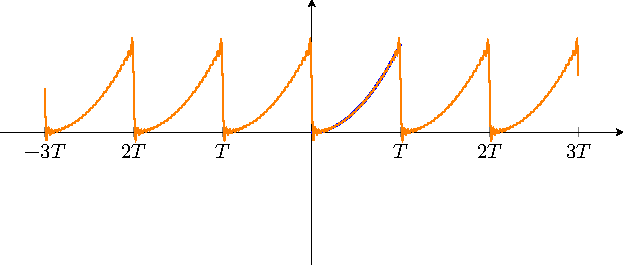
\includegraphics[width = 0.8\linewidth]{figures/half_range_expansion_Fourier.pdf}
    \caption{Fourier series expansion of \(f\left( t \right)\) on the interval \(\interval{0}{T}\), with the period \(T\).} % \label{}
\end{figure}
\begin{figure}[H]
    \centering
    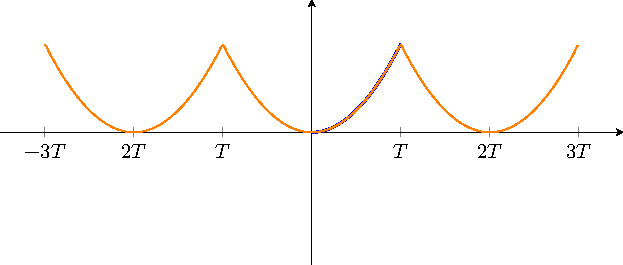
\includegraphics[width = 0.8\linewidth]{figures/half_range_expansion_Cosine.pdf}
    \caption{Fourier cosine series expansion of \(f\left( t \right)\) onto the interval \(\interval{-T}{T}\), with the period \(2T\).} % \label{}
\end{figure}
\begin{figure}[H]
    \centering
    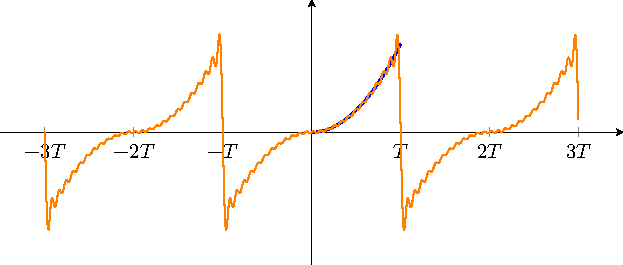
\includegraphics[width = 0.8\linewidth]{figures/half_range_expansion_Sine.pdf}
    \caption{Fourier sine series expansion of \(f\left( t \right)\) onto the interval \(\interval{-T}{T}\), with the period \(2T\).} % \label{}
\end{figure}
\end{document}
